
%=============================================================================
\section{Higher Level Components}
\label{sec:ddg4-implementation-higher-level-components}
%=============================================================================
\noindent
Layered components, which base on the general framework implement higher 
level functionality such as the handling of Monte-Carlo truth associations
between simulated energy deposits and the corresponding particles or the
generic handling of input to the simulation.

\noindent
To generalize such common behavior it is mandatory that the participating
components collaborate and understand the data components they commonly access.
The data model is shown in Figure~\ref{fig:ddg4-event-data-model}.
\begin{figure}[t]
  \begin{center}
    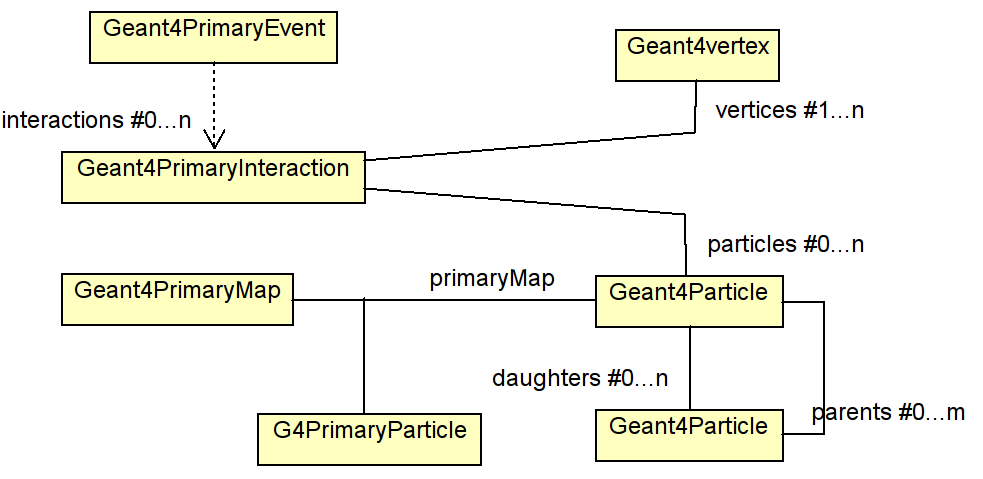
\includegraphics[width=120mm] {DDG4_event_data_model}
    \caption{The DDG4 event data model.}
    \label{fig:ddg4-event-data-model}
  \end{center}
\end{figure}

\noindent
{\bf{Please note}}, that this data model  is by no means to be made persistent 
and used for physics user analysis. This model is optimized to support
the simulation process and the necessary user actions to handle MC truth,
to easily and relatively fast look up and modify parent-daughter 
relationships etc. This choice is based on the assumption, that the 
additional overhead to convert particles at the input/output 
stage is small compared to the actual resource consumption of Geant4
to simulate the proper detector response.
On the other hand this choice has numerous advantages:
\begin{itemize}\itemcompact
\item Accepting the fact to convert input records allows to adapt 
  DDG4 in a simple and flexible manner to any input format. Currently 
  supported is the input from raw {\tts{LCIO}} files, {\tts{StdHep}} 
  records using {\tts{LCIO}} and {\tts{ASCII}} files using the 
  {\tts{HEPEvt}} format.
\item Similarly as for the input stage, also the output format 
  can be freely chosen by the clients.
\item No assumptions was made concerning the structure to store 
  information from energy deposits. Any information extract produced
  by the sensitive actions can be adapted provided at the output
  stage the proper conversion mechanism is present. The sensitive 
  detectors provided by DDG4 are {\bf{optional only and by no means mandatory}}.
  User defined classes may be provided at any time. Appropriate tools
  to extract MC truth information is provided at the output stage.
\item The modular approach of the action sequences described 
  in~\ref{sec:ddg4-user-manual-implementation-geant4action-sequences}
  allows to easily extend the generation sequence to handle multiple 
  simultaneous interactions, event overlay or spillover response 
  very easily~\footnote{The handling of spillover is only possible 
  if during the digitization step the correct signal shape corresponding
  to the shift of signal creation is taken into account.}
\end{itemize}

\noindent
In section~\ref{sec:ddg4-implementation-input-handling} the generic mechanism
of input data handling is described. \\
In section~\ref{sec:ddg4-implementation-particle-handling} the MC truth 
handling is discussed. \\
In section~\ref{sec:ddg4-implementation-output-handling} we describe the 
output mechanism.
\newpage

%=============================================================================
\subsection{Input Data Handling}
\label{sec:ddg4-implementation-input-handling}
%=============================================================================
\begin{figure}[t]
  \begin{center}
    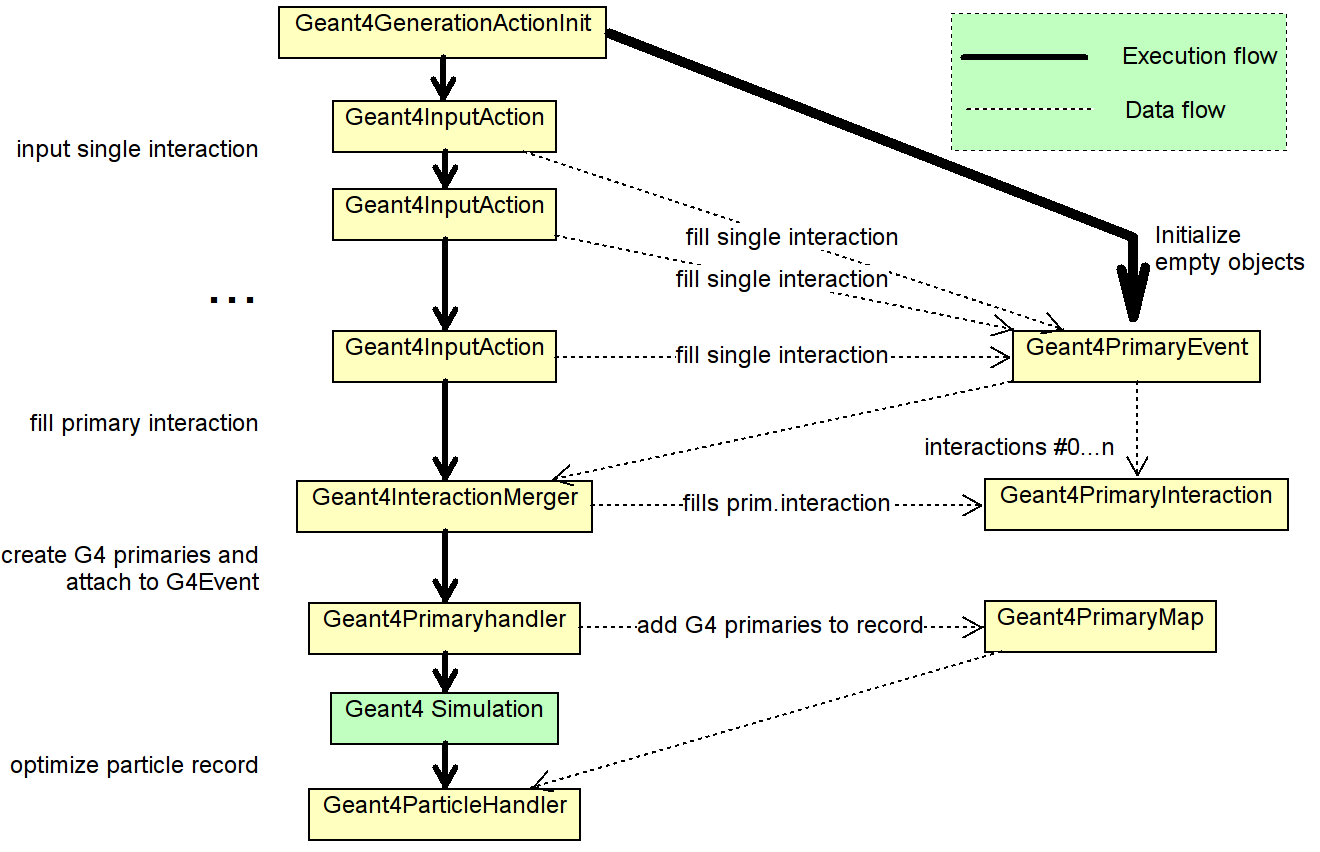
\includegraphics[width=160mm] {DDG4_input_stage}
    \caption{The generic handling of input sources to DDG4.}
    \label{fig:ddg4-input-stage}
  \end{center}
\end{figure}

\noindent
Input handling has several stages and uses several modules:
\begin{itemize}\itemcompact
\item First the data structures \tts{Geant4PrimaryEvent}, 
    \tts{Geant4PrimaryInteraction} and \tts{Geant4\-Primary}\-\tts{Map} are initialized 
    by the action \tts{Geant4GenerationActionInit} 
    and attached to the {\tts{Geant4Event}} structure.
\item The initialization is then followed by any number of input modules.
  Typically each input module add one interaction. Each interaction has a 
  unique identifier, which is propagated later to all particles. Hence all
  primary particles can later be unambiguously be correlated to one of the 
  initial interactions. 
  Each instance of a \tts{Geant4InputAction} creates and fills a separate instance
  of a \tts{Geant4PrimaryInteraction}.
  In section~\ref{sec:ddg4-implementation-geant4inputaction} the functionality and
  extensions are discussed in more detail.
\item All individual primary interactions are then merged to only single record
  using the \tts{Geant4}\-\tts{Interaction}\-\tts{Merger} component.
  This components fills the \tts{Geant4PrimaryInteraction} registered to the
  \tts{Geant4Event}, which serves as input record for the next component,
\item the \tts{Geant4PrimaryHandler}. The primary handler creates the proper 
  \tts{G4PrimaryParticle} and \tts{G4PrimaryVertex} objects passed to \tts{Geant4}.
  After this step all event related user interaction with Geant4 has completed,
  and the detector simulation may commence.
\end{itemize}
All modules used are subclasses of the {\tts{Geant4}\-\tts{Generator}\-\tts{Action}} and must be
added to the \tts{Geant4}\-\tts{Generator}\-\tts{Action}\-\tts{Sequence} as described 
in~\ref{sec:ddg4-user-manual-implementation-geant4action-sequences}.

\noindent
An object of type {\tts{Geant4PrimaryEvent}} exists exactly once for 
every event to be simulated. The empty {\tts{Geant4PrimaryEvent}} is created by the
{\tts{Geant4GenerationActionInit}} component. All higher level components may then 
access the {\tts{Geant4PrimaryEvent}} object and subsequently an individual interaction
from the {\tts{Geant4Context}} using the extension mechanism as shown in 
the following code:
\begin{code}
/// Event generation action callback
void SomeGenerationComponent::operator()(G4Event* event)  {
  /// Access the primary event object from the context
  Geant4PrimaryEvent* evt = context()->event().extension<Geant4PrimaryEvent>();
  /// Access the container of interactions
  const std::vector<Geant4PrimaryEvent::Interaction*>& inter = evt->interactions();
  /// Access one single interaction to be manipulated by this component
  Geant4PrimaryInteraction* evt->get(m_myInteraction_identifier);
  ....
\end{code}
{\bf{Please note:}} To keep components simple, each component should 
only act on one interaction the component has to uniquely identify.
The identification may be implemented by e.g. an access mask passed to the 
component as a property.

%=============================================================================
\subsection{Anatomy of the Input Action}
\label{sec:ddg4-implementation-geant4inputaction}
%=============================================================================
\noindent
One input action fills one primary interaction.
\tts{Geant4InputAction} instances may be followed by decorators, which 
allow to to smear primary vertex (\tts{Geant4InteractionVertexSmear}) or
to boost the primary vertex \tts{Geant4InteractionVertexBoost} and all 
related particles/vertices.


Please note, that a possible reduction of particles in
the output record may break this unambiguous relationship between 
"hits" and particles.
......

%=============================================================================
\subsection{Monte-Carlo Truth Handling}
\label{sec:ddg4-implementation-particle-handling}
%=============================================================================
......
\newpage

%=============================================================================
\section{Output Data Handling}
\label{sec:ddg4-implementation-output-handling}
%=============================================================================
......
\newpage
